\documentclass{thesisreport}

\usepackage{caption}
\usepackage{subcaption}
\usepackage{comment}

\begin{document}

 \thispagestyle{empty}

\def\lskip{\vspace{0.5cm}}


\begin{tabular}{p{7cm}p{8cm}}
ÉCOLE CENTRALE DE NANTES
&
% EMARO students only
% \raggedleft FIRST YEAR INSTITUTION	
\end{tabular}

\vspace{2cm}

% CORO-IMARO students
\begin{center} \large\sc MASTER CORO-IMARO\\ \normalsize{``CONTROL and ROBOTICS''} \end{center}

% EMARO students
%\begin{center} \large\sc MASTER ERASMUS MUNDUS \\ \normalsize{EMARO+ ``European Master in Advanced Robotics''} \end{center}


\begin{center}
	2016 / 2017\\
	\lskip
	Master Thesis Report % or bibliography report
	\lskip
	
	Presented by \lskip 
	
	Student Name \lskip
	
	On Date \lskip\lskip
	
	{\Large \textbf{The title of the master thesis}}
	
	\vfill

Jury \lskip
		
	\end{center}
	


\begin{tabular}{p{3cm}p{7cm}p{5cm} }
 % President: & Name & Position (Institution) \\ & & \\     % for final defense only (not bibliography)
 Evaluators: & Name & Position (Institution) \\
	      & Name & Position (Institution) \\ 
	      & Name & Position (Institution) \\ & & \\  & & \\ 
  Supervisor(s):  & Name & Position (Institution) \\
		  & Name & Position (Institution) \\
% EMARO students only
%(EMARO)  & Co-supervisor from M1 & Position, M1 institution 
\end{tabular}

\lskip

\begin{flushleft}
 Laboratory: Laboratoire des Sciences du Numérique de Nantes LS2N
\end{flushleft}

\newpage
\thispagestyle{empty}
\null
\newpage
\addtocounter{page}{-1}
\pagestyle{fancy}
  
 
  \section*{Abstract}
Within the rapidly growing aerial robotics market, one of the most substantial challenges in the quadrotor community is performing aggressive maneuvers, especially multi-flip maneuvers.  A proper physical definition of the issue is not addressed by the current approaches in the field and several key aspects of this maneuver are still overlooked.
It can be shown, in particular, that making a flip with a quadrotor means crossing the parallel singularity of the dynamic model. The aim of the master thesis is to explore the possibility of defining aggressive trajectories for quadrotors on the basis of their dynamic model degeneracy analysis and to adapt various strategies to control the robot in a closed loop. In addition, the possibility to perform the aggressive maneuver in constrained environments will also be investigated.
Therefore, the analysis will be extended from the previous studied to create general feasible trajectories that will allow quadrotors to perform aggressive flip maneuvers while passing through a constrained environment and while guaranteeing a satisfactory degree of robustness to the uncertainties of the dynamic model.

 
 \newpage
 
 \section*{Acknowledgements}


I would like to express my special thanks and gratitude to my supervisors Dr. Sébastien Briot and Dr. Isabelle Fantoni who gave me the  opportunity to work on this wonderful project which encapsulates control theory, dynamics and quadrotors. This project has allowed me to perform research on all of these topics and I am now more knowledgeable thanks to my supervisors. Moreover, I would like to thank them for believing in my capabilities and for me the confidence when I needed it. \\

Secondly, I would also like to thank Dr. Ina Taralova for providing me with the valuable knowledge to create a proper bibliography. \\


I would like to thank my patient and understanding girlfriend Glysa, who has been with me for more than 5 years. Thank you for all the love, support and comfort that you have given me in these stressful 2 years. I hope that this Master degree will allow us to have a better future together. \\


I would like to thank my family as well: my parents Naji and Yolla, my sister Rebecca, my uncle and his wife Fadi and Lara and my aunt Bernadette. They have provided me with the emotional and economical support from the very beginning and they gave me the opportunity to travel and study for this Master degree. They have always been proud and encouraging. I would not be here if it wasn't for them.

 
 \newpage
 
 
 \section*{Notations}
 
 \newpage
 
  \section*{Abbreviations}
 
 \newpage
 
 \listoffigures
 
\listoftables
 
 \tableofcontents
 
 
 \chapter*{Introduction}
 \addcontentsline{toc}{chapter}{Introduction}	 % non-numbered chapters do not appear in table of contents by default
 	The aim of this section is to provide a general summary of the robotic robotic platform that is used for this master thesis and to illustrate the main objective of the research work.
In specific, in the sections below, quadrotors and parallel robots are briefly presented.


 
 
\section*{The quadrotor platform}

A quadrtor is a type of unmanned aerial vehicle with four rotors and six degrees of freedom. Typically, drones have a small size and low inertia which allows it to be controller by simple flight control systems. It is typically designed in a cross-configuration such that the electronics are held in the center of the platform and the rotors are placed at the borders.
An example of a real quadrotor, namely the DJI Phantom, is shown in fig. \ref{fig:drone}. The quadrotor is typically built in a way such that a pair of opposite rotors rotate clockwise, whereas the other pair of rotors rotates in counter-clockwise.
The attitude and the position of the drone are controlled by changing the spinning speed of the rotors. An example is shown in figure \ref{fig:propeller_directions}.



\begin{figure}[h]
     \centering
     \begin{subfigure}[b]{0.45\textwidth}
         \centering
         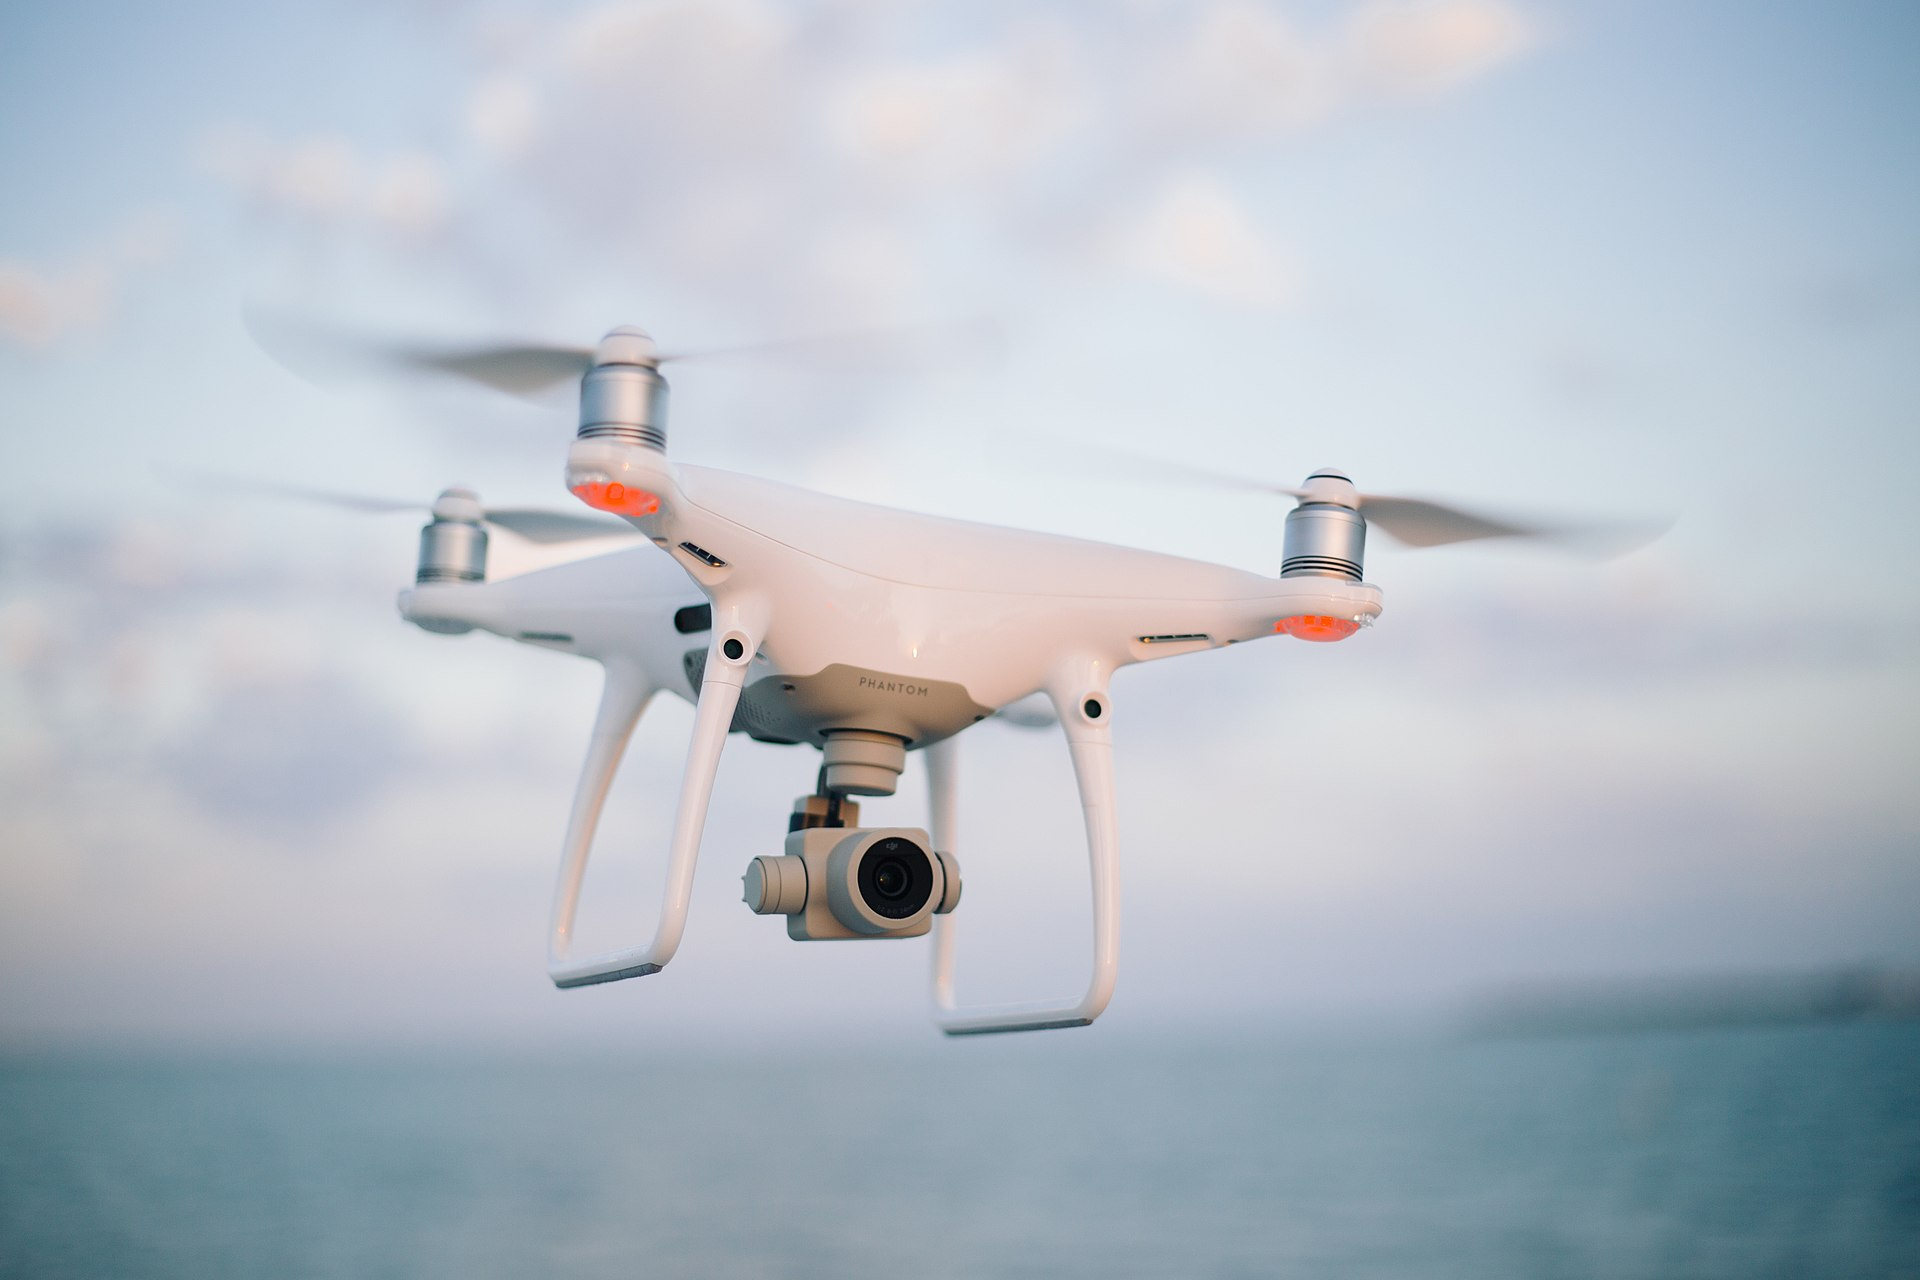
\includegraphics[width=\textwidth]{Images/Introduction/drone}
    \caption{A DJI Phantom quadcopter (UAV)}
         \label{fig:drone}
     \end{subfigure}
     \hfill
     \begin{subfigure}[b]{0.45\textwidth}
         \centering
         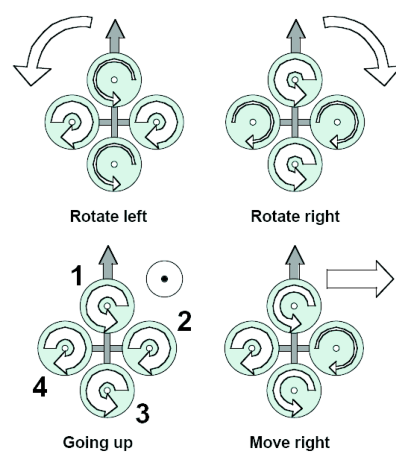
\includegraphics[width=0.6\textwidth]{Images/Introduction/propeller_direction.svg}
         \caption{Typical quadrotor configuration The width of the arrows is proportional to the angular speed of the propellers. \cite{Bouabdalla2007}}
         \label{fig:propeller_directions}
     \end{subfigure}
        \caption{A commercial quadrtotor platform, with a typical quadrotor configuration.}
        \label{fig:three graphs}
\end{figure}











 \chapter{State of the art}
 
 \section{First topic}
 
 \section{Second topic}
 
 \chapter{Actual work}
  
 
 When dealing with rectangled triangles (see Figure \ref{triangle}) I sometimes used this theorem from \cite{pythm001}:
 \begin{equation}\label{theo}
  a^2 + b^2 = c^2
 \end{equation}The demonstration is in Appendix \ref{sec:prooftheorem}.
 
 \begin{figure}[h]\centering
  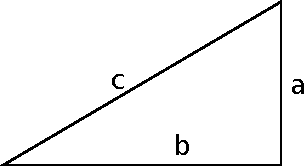
\includegraphics[width=.5\linewidth]{triangle1}
  \caption{A triangle with letters} \label{triangle}
 \end{figure}
 
 


 
 
 \chapter{Experiments}
 
 When trying to draw a rectangled triangle, my program comes up with Figure \ref{triangle2} that is neither rectangled nor a triangle.
 
  \begin{figure}[h]\centering
  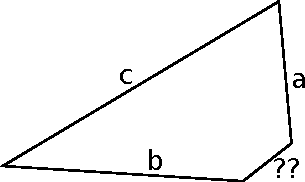
\includegraphics[width=.5\linewidth]{triangle2}
  \caption{Triangle drawn by my program. Note the 4th side.} \label{triangle2}
 \end{figure}
 
Unless there is a bug in my program, which is unlikely, this research indicates that the whole theory on triangles having 3 sides has been wrong for years, maybe decades. \cite{Bouabdalla2007}
 
 
 \chapter*{Conclusion}
 \addcontentsline{toc}{chapter}{Conclusion}
 
 
 
 

 % switch to A-B-C chaptering
 \appendix	
 
 \chapter{Proof of theorem \ref{theo}}
 \label{sec:prooftheorem}
  
 \begin{proof}
 was already demonstrated in \cite{Bouabdalla2007}.
\end{proof}

 \addcontentsline{toc}{chapter}{Bibliography}
 \nocite{*}
 
 \bibliography{../biblio}

 
 
\end{document}
